%%% Ne pas modifier jusqu'à la ligne 25
\documentclass[a4paper,12pt]{book}
\usepackage[utf8]{inputenc}
\usepackage[french]{babel}
%%\usepackage{CJK}
\usepackage{yhmath}
\usepackage[left=2cm,right=2cm,top=3cm,bottom=2cm, headheight=1.5cm,headsep=1.5cm]{geometry}
%%\usepackage{CJKutf8}
\usepackage{amsfonts}
\usepackage{mathrsfs}
\usepackage{amsmath,amsfonts,amssymb,dsfont}
\usepackage{graphicx}
\usepackage{subfigure}
\usepackage{enumitem}		%\enumerate-resume
\usepackage[colorlinks=true,unicode={true},hyperindex=false, linkcolor=blue, urlcolor=blue]{hyperref}
\newcommand{\myref}[1]{\ref{#1} page \pageref{#1}}

\addto\captionsfrench{\def\tablename{Tableau}}  %légendes des tableaux
\renewcommand\thesection{\Roman{section}~-~} 
\renewcommand\thesubsection{\Roman{section}.\Alph{subsection}~-~} 
\renewcommand\thesubsubsection{\Roman{section}.\Alph{subsection}.\arabic{subsubsection}~-~} 

\newcommand{\conclusion}[1]{\newline \centerline{\fbox{#1}}}

\setcounter{secnumdepth}{3}
\parindent=0pt

\usepackage{fancyhdr}
\pagestyle{fancy}

\lhead{SJTU-ParisTech} 
%%%%%%%%%%%%%%%%%%%%%%%%%%%%%%%%%%
\chead{TR11}
\rhead{Daniel 518261910024}
\begin{document}
\renewcommand{\labelitemi}{$\blacktriangleright$}
\renewcommand{\labelitemii}{$\bullet$}


\section{figures d’interférences}
Les figures sont obtenues par une superposition de $N$ ondes, avec $N$ varié.
Par notre simplification que leur amplitudes sont identique au point $M$ étudié, et que 
le déphasage entre les rayons issues de $S_{m+1}$ et $S_m$ est une constante au $M$, 
on a 
$$
\mathcal{E}(M)=\mathcal{E}_0\left(\frac{\sin \frac{N\delta \phi}{2}}{\sin \frac{\delta \phi}{2}}\right)^2
$$
\begin{itemize}
    \item Figure 1. On notice que la largeur des franges brillantes égale à celle des franges sombres, 
          cette figure est plutôt pour une éclairement qui varie sinusoïdalement: Le cas pour la superposition 
          de deux ondes cohérentes. 
          \begin{figure}[h]
            \begin{center}
            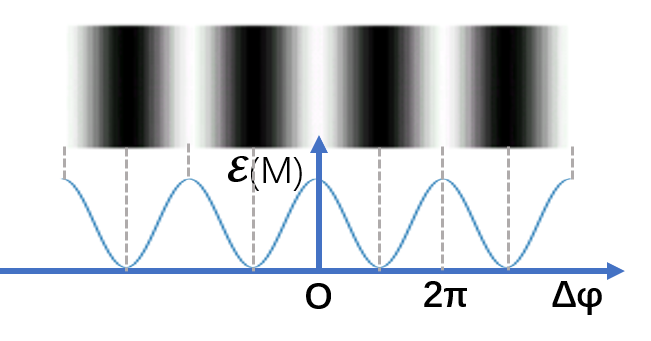
\includegraphics[scale=0.8]{tr111.png}
            \end{center}
            \vspace{-0.8cm}
            \caption{éclairement de Figure 1}
        \end{figure}
    


    \item Figure 2. C'est exactement ce que nous avons vu en cours: il y a des maxima secondaires qui sont moins lumineuses que 
          les maxima principaux. 

          On sait que la largeur d'un pic principal $\delta_{pp}=\frac{4\pi}{N}$. Car la figure est $2\pi-\mbox{périodique}$, 
          on a $\pi=\delta_{pp}=\frac{4\pi}{N}$, d'où $N=4$. Figure 2 est donc une superposition de $4$ ondes cohérentes
          \begin{figure}[h]
            \begin{center}
            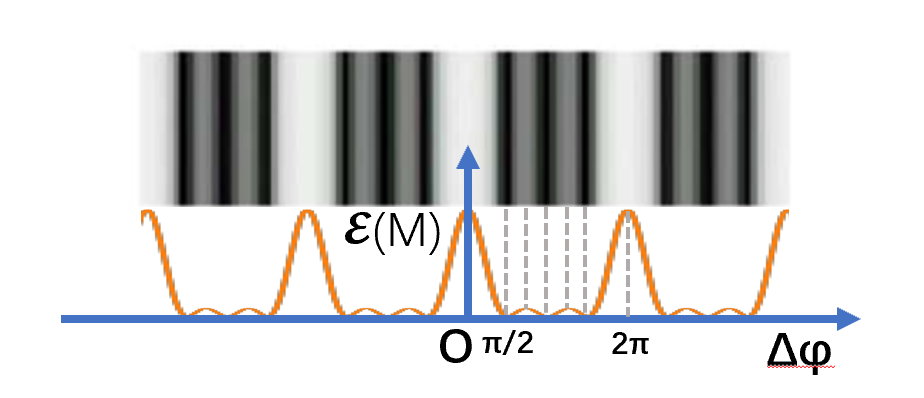
\includegraphics[scale=0.8]{tr112.png}
            \end{center}
            \vspace{-0.8cm}
            \caption{éclairement de Figure 2}
        \end{figure}


    \item Figure 3. On sait que les maxima secondaires sont de moins en moins visibles lorsque $N$ augmente, et les maxima principaux 
          sont de plus en plus fins(car $\delta_{pp}=\frac{4\pi}{N}$), c'est le cas pour Figure 3.
    



    \item Figure 4. Pour Figure 4, la frange brillante est la plus fin. 
          On sait que les maxima principaux sont de plus en plus fins et les maxima
          secondaires sont de plus en plus petits lorsque N augmente, c'est exactement 
          le cas de Figure 4 pour $N$ très élevé.   


\end{itemize}
En conclusion, ils sont tous obtenus par la superposition de $N$ ondes, comme nous avons vue en cours. 
On peut obtenir la figure d'interférence comme Figure 1 à celle comme Figure 4 en augmentant $N$. 
\end{document}